%% LyX 1.1 created this file.  For more info, see http://www.lyx.org/.
%% Do not edit unless you really know what you are doing.
\documentclass[10pt,english]{article}
\usepackage{pslatex}
\usepackage[T1]{fontenc}
\usepackage[latin1]{inputenc}
\usepackage{babel}
\setlength\parskip{\medskipamount}
\setlength\parindent{0pt}
\usepackage{graphics}
\usepackage{floatflt}
\IfFileExists{url.sty}{\usepackage{url}}
                      {\newcommand{\url}{\texttt}}

\makeatletter

%%%%%%%%%%%%%%%%%%%%%%%%%%%%%% LyX specific LaTeX commands.
\providecommand{\LyX}{L\kern-.1667em\lower.25em\hbox{Y}\kern-.125emX\@}

%%%%%%%%%%%%%%%%%%%%%%%%%%%%%% Textclass specific LaTeX commands.
 \newenvironment{lyxcode}
   {\begin{list}{}{
     \setlength{\rightmargin}{\leftmargin}
     \raggedright
     \setlength{\itemsep}{0pt}
     \setlength{\parsep}{0pt}
     \normalfont\ttfamily}%
    \item[]}
   {\end{list}}

\makeatother
\begin{document}

\title{Configuring Perdition Proxy Software to Use An Existing LDAP Server}


\author{Richard L. Holbert}

\maketitle

\part*{Introduction}

The Perdition proxy server software was designed by Simon Horman as
part of a high availability email system. Perdition allows an ISP
to distribute end user mail boxes over several servers seamlessly.
All the end users connect through the proxy server(s) to retrieve
their email via POP, and/or IMAP. User redirection information can
be stored using a variety of methods including: gdbm, NIS, regular
expressions, relational data bases (MySQL, PostgreSQL), and LDAP.

The main perdition web site is \url{http://www.vergenet.net/linux/perdition/}

The author's email address is: horms@vergenet.net

Perdition also requires that the VAnessa (VA Network Enhanced Scalable
Server Architecture) libraries be installed. The VAnessa web site
is at: \url{http://www.vergenet.net/linux/vanessa/}. Both sets of
tools were downloaded from: ftp.vergenet.net, and installed on my
Linux workstation using the Redhat Package Manager (RPM). In a production
environment, Perdition and VAnessa should be installed on a set of
dedicated servers.

Perdition comes with a tool to populate an empty OpenLDAP server with
its default schema, perditiondb\_ldap\_makedb. However, as we already
have several existing, populated, iPlanet LDAP servers along with
an infrastucture to maintain the information in them, I decided to
adapt Perdition to use our existing servers' schemas. 


\part*{LDAP URLs}

Perdition extracts information from LDAP via specially configured
URLs.

LDAP URLs are documented in RFC 2255 \url{http://www.cis.ohio-state.edu/cgi-bin/rfc/rfc2255.html},
and the iPlanet Directory Server Administrator's Guide (Appendix C)
\url{http://docs.iplanet.com/docs/manuals/directory/51/html/ag/url.htm#1915312}.

LDAP URLs have the following format:

ldap{[}s{]}://hostname{[}:port{]}/search\_base?attributes?scope?filter

Cleartext connections are made using the ldap:// protocol, and encrypted
(SSL) conections are made using the ldaps:// protocol.

{\centering LDAP URL Components:\par}

\begin{tabular}{|l|l|}
\hline 
\multicolumn{1}{|p{1.0in}|}{Component}&
\multicolumn{1}{p{4.5in}|}{Definition}\\
\hline
\hline 
\multicolumn{1}{|l|}{hostname}&
\multicolumn{1}{p{4.5in}|}{\noindent \raggedright Server name, or numerical ip address. Example,
ldap.mydomain.edu, or 10.10.220.90}\\
\hline 
port&
\multicolumn{1}{p{4.5in}|}{The LDAP service's port number. Example, 389, or 636 if using the
secure (ldaps) protocol. A blank here defaults to 389 for ldap, and
636 for ldaps.}\\
\hline 
search\_base&
\multicolumn{1}{p{4.5in}|}{Consists of an entry's distinguished name (DN). The search\_base tells
Perdition where to start its search.}\\
\hline 
attributes&
\multicolumn{1}{p{4.5in}|}{Names of the LDAP fields to be returned. A blank here returns all
visible attributes. The port attribute is optional if standard POP3,
and IMAP4 ports are being used.}\\
\hline 
scope&
\multicolumn{1}{p{4.5in}|}{Scope consists of one of the following: base, one, or sub. For all
the schemas tested, Perdition seems to work with either one, or sub,
but not with base.}\\
\hline 
filter&
\multicolumn{1}{p{4.5in}|}{Criteria to be used within the scope of the search. Example, (uid=\%25s).
The \%25s gets replaced with the userid supplied by the user's email
client.}\\
\hline
\end{tabular}



\part*{Configuration}

Recommended configuration approach: via changes to /etc/perdition/perdition.conf
file. To configure Perdition to use LDAP, add the following lines:

M /usr/lib/libperditiondb\_ldap.so

m ldap://hostname.mydomain.com:port/ou=mailbox,dc=mydomain.com,dc=com?user-name,mailhost,port?one?(uid=\%25s)

Substitute your server's name, ldap port, search\_base, etc.

Another approach is to modify perditions startup script by appending
the -M and -m values from above to the proxies command line.


\part*{Rapid Testing}

A web browser, such as Netscape, Konqueror, Mozilla, etc. can be used
in conjunction with a GUI LDAP tool, like GQ, to derive and test LDAP
queries.

The ficticious iplanet-ldap server uses iPlanet's messaging server
schema.

The following is a screen shot of iplanet-ldap's tree structure.

\vspace{0.3cm}
{\centering \resizebox*{5in}{3in}{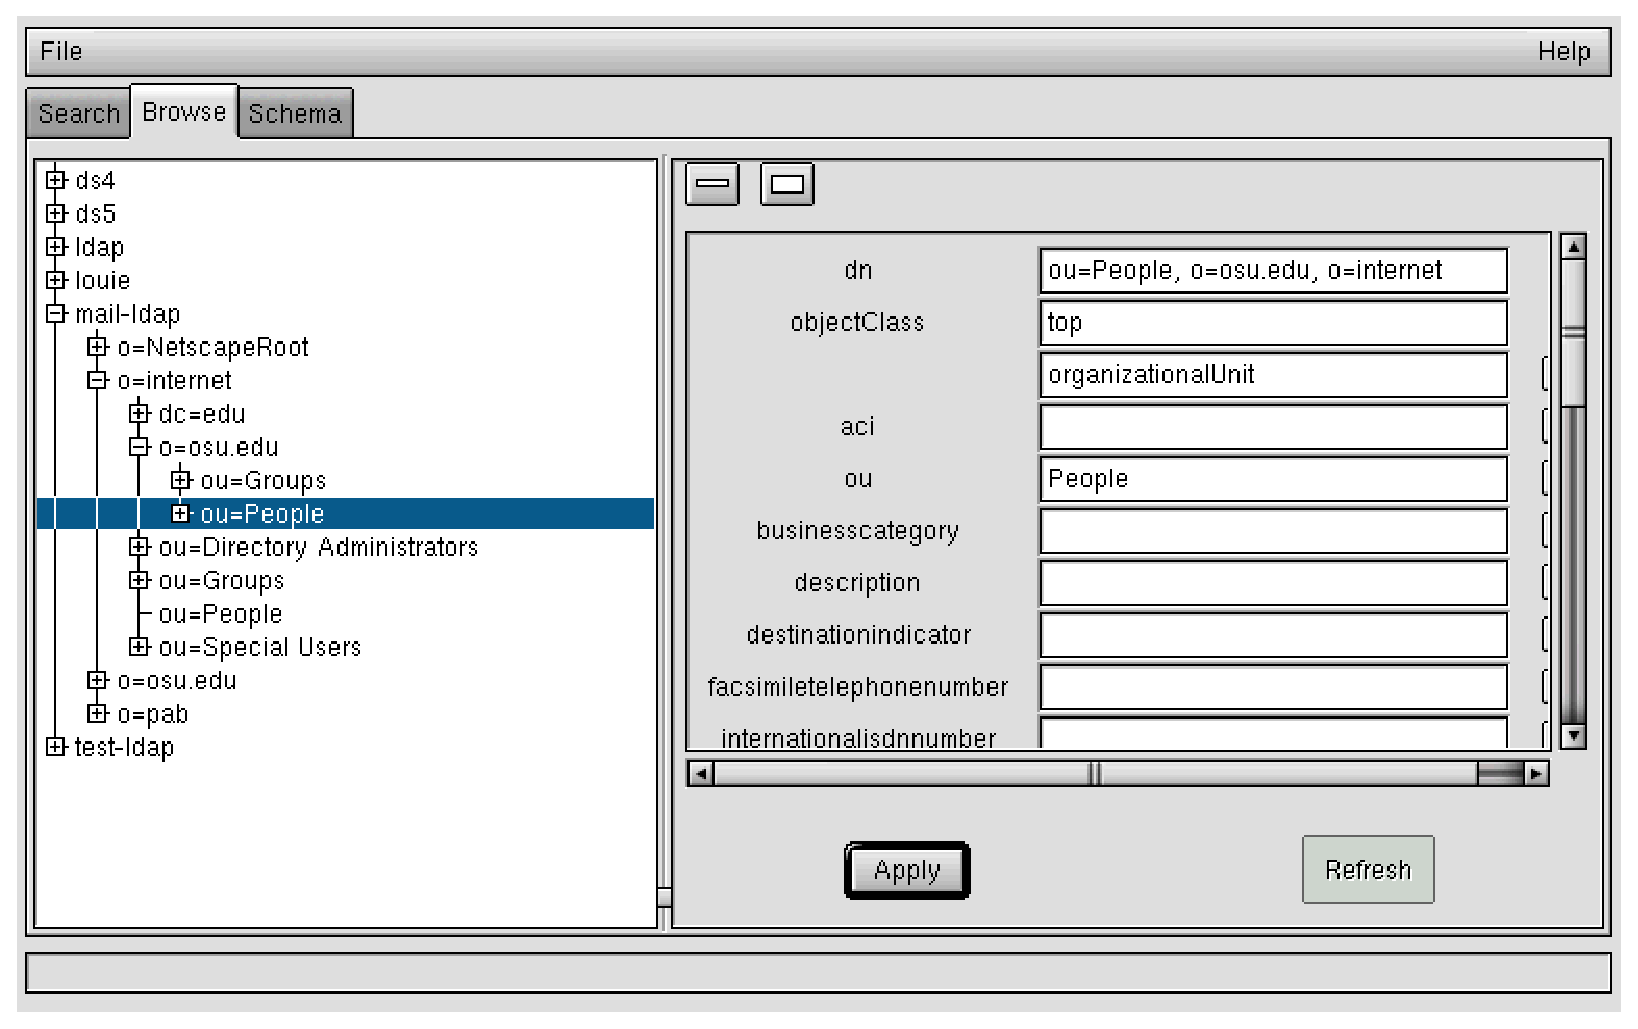
\includegraphics{mail-ldapdump.eps}} \par}
\vspace{0.3cm}

However, directoryserver4, and directoryserver5 use a modified eduPerson
schema. As a result, the search bases differ.

Here's a screen shot of directoryserver5's tree structure.

\vspace{0.3cm}
{\centering \resizebox*{5in}{3in}{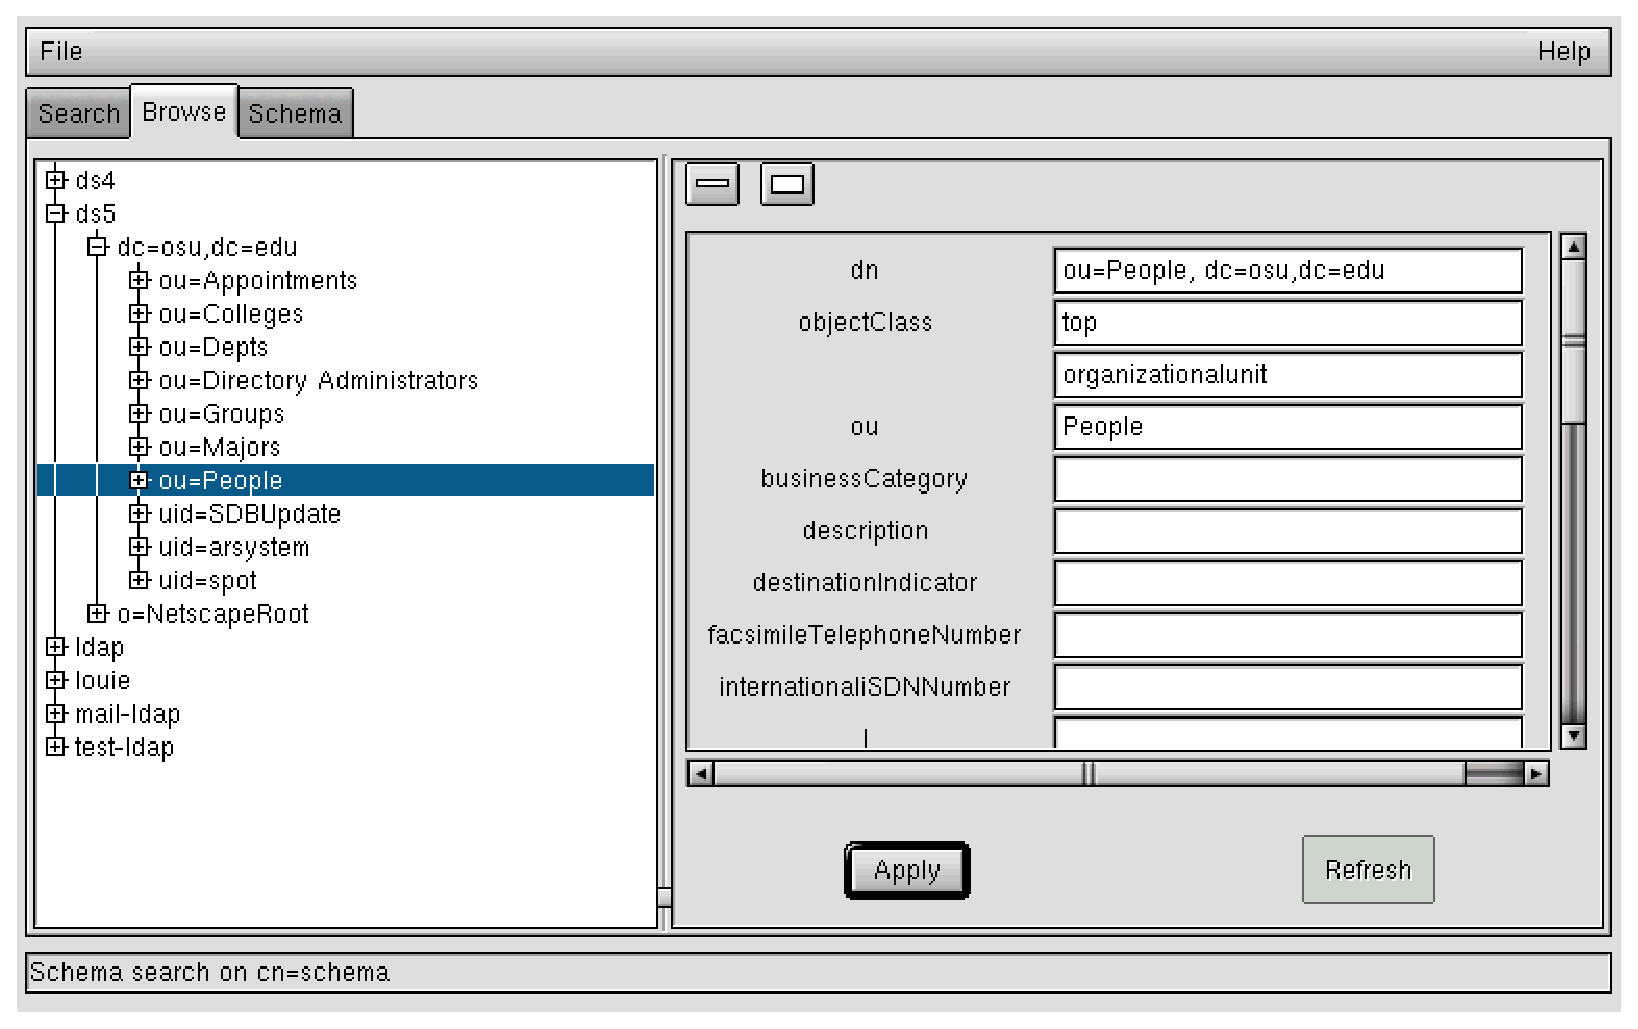
\includegraphics{ds5dump.eps}} \\
\par}
\vspace{0.3cm}

The access controlls for directoryserver5 had to be modified to make
the mailhost attribute visible from anonymous binds.

Some example LDAP queries along with their results are as follows:

ldap://iplanet-ldap.mydomain.edu:389/ou=people,o=mydomain.edu,o=internet?uid,mailhost?one?(uid=smith.13)

\begin{lyxcode}
dn:~uid=smith.13,ou=People,~o=mydomain.edu,~o=internet

uid:~smith.13

mailhost:~mail2.service.mydomain.edu
\end{lyxcode}
ldap://directoryserver5.service.mydomain.edu:20389/ou=people,dc=osu,dc=edu?uid,mailhost,port?one?(uid=jones.6)

\begin{lyxcode}
dn:~mydomainEduID=397427,~ou=People,~dc=mydomain,~dc=edu

uid:~jones.6

mailhost:~mail1.service.mydomain.edu
\end{lyxcode}
Notice how the order of the search base dn starts with the bottom
of the tree, and works its way back up the tree. Also note that in
this example, directoryserver5 uses non-standard port, 20389 for LDAP.


\part*{Extensions}

The basic LDAP URL can be extended in two ways.

If the LDAP servers are using standard ports, then multiple servers
can be used in the LDAP URL. For example:

ldap://ldap1 ldap2 ldap3/ou=people,o=mydomain.edu,o=internet?uid,mailhost,port?one?(uid=smith.13)

So far, all the examples have used anonymous binds to connect to the
LDAP servers. The LDAP URL may be extended using the bindname, and
x-bindpw attributes as follows:

ldap://ldap1:389/ou=people,o=mydomain.edu,o=internet?uid,mailhost,port?one?(uid=smith.13)?!\\
bindname=cn=admin,x-bindpw=secret

or

ldaps://secure-ldap:636/ou=people,o=mydomain.edu,o=internet?uid,mailhost?one?(uid=smith.13)?!\\
bindname=cn=super\%20admin,x-bindpw=bigsecret


\part*{Testing}

I conducted several tests using telnet, and a reconfigured email client.
I was able to retrieve mail from any of our existing mail servers
by pointing my email client at the Perdition proxy running on localhost.
Changing the value of my mailhost attribute in LDAP caused the proxy
to redirect my retrieval requests to the appropriate mail server.
\end{document}
